\documentclass[12pt, a4paper]{report}
\usepackage[utf8]{inputenc}
\newcommand\preamble{
    \usepackage[italian]{babel}
    \usepackage{geometry}
    \usepackage{amsmath}
    \usepackage{amssymb}
    \usepackage{graphicx}
    \usepackage{ulem}
    \geometry{margin=2cm}
    \usepackage{listings}
    \usepackage{xcolor}
    \let\olditemize\itemize
    \renewcommand\itemize{\olditemize\setlength\itemsep{0em}}
}
% Definizione delle variabili
\newcommand{\imagePath}{Immagini/logoUni.png}

% Definizione del comando per la pagina di titolo con argomenti
\newcommand{\customTitlePage}[2]{
    \newcommand{\courseTitle}{#1}
    \newcommand{\academicYear}{#2}
    
    \begin{titlepage}
        \centering
        \includegraphics[width=0.5\textwidth]{\imagePath}\par\vspace{1cm}
        {\scshape\LARGE University of Studies of Genoa \par}
        \vspace{1.5cm}
        {\huge\bfseries \courseTitle \par}
        \vspace{2cm}
        {\Large\itshape Lorenzo Vaccarecci \par}
        \vfill
        \academicYear
    \end{titlepage}
}

\preamble

\begin{document}
\customTitlePage{Computer Security}{2024-2025}
\newpage
\tableofcontents
\chapter{Introduction}
Computer security deals with the preventon and detection of unauthorized actions by users of a computer system.
\begin{itemize}
    \item \textbf{Authorization} is central to definition
    \item Sensible only relative to a security policy, stating who (or what) may perform which actions
\end{itemize}
\section{Information Security}
Is even more general. It deals with information independent of computer security.
\subsection{Key Concepts}
\begin{itemize}
    \item Security concerns the protection of assets from threats
    \item Owners value their assets and want to protect them
    \item Threat agents also value assets, and seek to abuse them
    \item Owners analyse threats to determine which ones apply; these are the risks that can be costed. This helps the selection of countermeasures, which reduce the vulnerabilities (may remain leaving some residual risk, owners seek to minimise that risk)
\end{itemize}
\begin{equation*}
    \text{Risk}_{E} = \text{Pr}_{E} \cdot \text{I}_{E}
\end{equation*}
where $\text{Pr}_{E}$ is the probability of an event $E$ and $\text{I}_{E}$ is the impact of the event $E$.
\section{Protection countermeasures}
\begin{itemize}
    \item \textbf{Prevention}: try to prevent security breaches by system design and employing appropriate security technologies as defences
    \item \textbf{Detection}: in the event of a security breach, we try to ensure that it will be detected. Logging and MACs (file hashes to detect alteration)  are primary methods of detection, although intrusion detection systems which activelyy watch for intruders are more common
    \item \textbf{Response}: in the event of a security breach, we must respond or recover the assets. Responses range from restoring backups through to informing appopriate concerned parties or law-enforcement agencies
\end{itemize}
\section{Security Properties}
\subsection{Confidentiality}
\customfbox{Information is not learned by unauthorized principals}
Confidentiality is sometimes characterised as the unauthorized reading of data, when considering \textbf{access control} measures. But in general we are concerned with unauthorized learning of information, which is more subtle to contend with. Confidentiality presumes a security policy saying who or what can access our data. The security policy is used for access control.
\begin{itemize}
    \item \textbf{Privacy}: confidentiality for individuals
    \item \textbf{Secrecy}: confidentiality for organizations
    \item \textbf{Anonymity}: keeping one's identity private
\end{itemize}
\subsection{Integrity}
\customfbox{Data has not been maliciously altered}
Intergrity has more general meanings elsewhere, but in computer security we are concerned with preventing the possibly malicious alteration of data, by someone who is not authorized to do so. Integrity in this sense can be characterised as the unauthorized writing of data. Again, this presumes a security policy saying who or what is allowed to alter the data.
\subsection{Authenticity}
\customfbox{Data or services available only to authorized identities}
Authentication is th processo of verification of identity of a person or system. Some form of authentication is a pre-requisite if we wish to allow access to services or data to some people but deny access to others, using an access control system. Methods for authentication are often characterised as:
\begin{itemize}
    \item something you have
    \item something you know
    \item something you are
\end{itemize}
Also, where you are may be implicity or explicity checked. Several methods can be combined for extra security.
\subsection{Availability}
\customfbox{Data or services can be accessed in a reliable and timely way}
Threats to availability cover many kinds of external environmental events as well as accidental or malicious attackks in software. In computer security we're concerned with protecting against the second kind of threat, rather than providing more general forms of fault-tolerance or dependability assurance. Ensuring availability means preventing \textbf{denial od service} (DoS) attacks, insofar as this is possible. It's possible to fix attacks on faulty protocols, but attacks exhausting available resources are harder, since it can  be tricky to distinguish between an attack and a  legitimate use of service.
\subsection{Accountability}
\customfbox{Actions are recorded and can be traced to the party responsible}
If prevention methods and access controls fail, we may fall back to detection: keeping  a secure audit trail is important so that actions affecting security can be traced back to the responsible party. A stronger form of accountability is non-repudation, when a party cannot later deny some action. Creating an audit trail with machine logs is a tricky problem: if a system is compromised, the logs may also be tampered with. Ways around that problem are to send log messages to an append-only file, a separate server, or even a physically isolated printer.
\section{Implementing a security solution}
\begin{itemize}
    \item A \textbf{security analysis} surveys the threats which pose risks to assets, and then proposes policy and solutions at an appropriate cost.
    \item A \textbf{threat model} documents the possible threats to a system, imagining all the vulnerabilities which might be exploited
    \item A \textbf{riks assessment} studies the likelihood of each threat in the system environment and assigns a cost value, to find the risks
    \item A \textbf{security policy} addresses the threats, and describes a coherent set of countermeasures
\end{itemize}
The costs of countermeasures is compared against the risks, and juggles to make a sensible trade-off. This allows a security solution to be designed, deploying appropriate technologies at an appropriate cost. Partly this is a budgeting exercise; but it's also important to spend effort in the right place.
\chapter{Introduction to Cryptography}
How do we turn untrustworthy channels into trustworthy ones?
\begin{itemize}
    \item \textbf{Confidentiality}
    \item \textbf{Integrity}
    \item \textbf{Authenticity}
\end{itemize}
\section{General schema}
\begin{center}
    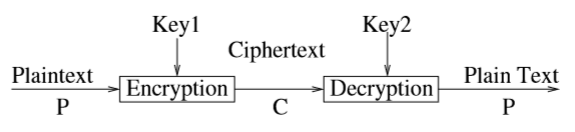
\includegraphics[width=.5\textwidth]{Immagini/schemacrittografia.png}
\end{center}
Where $E_{K_{1}}(P)=C, D_{K_{2}}(C)=P$
\begin{itemize}
    \item \textbf{Security depends on secrecy of the key, not of the algorithm}
    \item \textbf{Symmetric} algorithms: $K_{1}=K_{2}$ or are easily derived from each other
    \item \textbf{Asymmetric} or \textbf{public key} algorithms: different keys which cannot be derived  from each other and a \textbf{public key} can be published without compromising the \textbf{private key}
\end{itemize}
\begin{figure}[h]
    \centering
    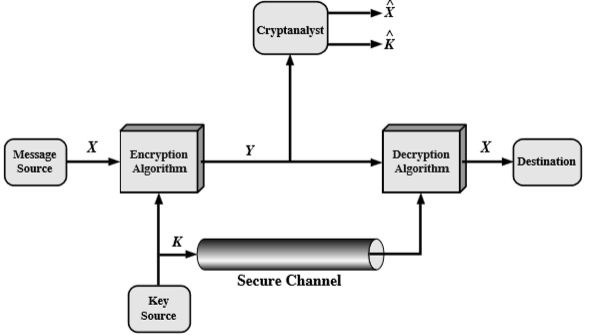
\includegraphics[width=.5\textwidth]{Immagini/chiavesimmetrica.png} 
    \caption{Model of Symmetric Cryptosystem}
\end{figure}
\section{Classification of security}
\begin{itemize}
    \item \textbf{Unconditional Security}: system is secure even if adversary has unbounded computing power since the ciphertext provides insufficient information to uniquely determine the corresponding plaintext. Security measured using information theory
    \item \textbf{Conditional Security}: system can be broken in principle, but  this requires more computing power than a realistic adversary would have. Security measured using complexity theory
\end{itemize}
\section{Cryptoanalysis}
\customfbox{Science of recovering the plaintext from ciphertext without the key}
But typical objective is to recover key not just message.
\subsection{Brute-force attack}
\begin{itemize}
    \item Always possible: try all possible keys ($2^{bit}$ number of keys)
    \item Its cost (eavily) depends on the key size
    \item It assumes that plaintext is known or recognisable
\end{itemize}
\subsection{Cryptanalytic attack}
\begin{itemize}
    \item \textbf{Ciphertext only}: only the ciphertext is known and the attacker tries to deduce the key
    \item \textbf{Known plaintext}: ciphertext only + plaintext
    \item \textbf{Chosen plaintext}: same as above but attacker can choose plaintext
    \item \textbf{Adaptive chosen plaintext}: cryptanalyst can not only choose plaintext, but he can modify the plaintext based on encryption results
    \item \textbf{Chosen ciphertext}: cryptanalyst can choose different ciphertexts to be decrypted and gets access to the decrypted plaintext
\end{itemize}
\section{Mathematical formalization}
\begin{itemize}
    \item $\mathcal{A}$: the alphabet
    \item $\mathcal{M}\subseteq\mathcal{A}$: the message space, $M\in\mathcal{M}$ is a plaintext
    \item $\mathcal{C}$: the ciphertext space, whose alphabet may differ from $\mathcal{M}$
    \item $\mathcal{K}$: the key space
    \item $\forall e\in\mathcal{K}$ determines a bijective function $E_{e}:\mathcal{M}\rightarrow\mathcal{C}$. $E_{e}$ is the encryption function
    \item $\forall d\in\mathcal{K}$ determines a bijective function $D_{d}:\mathcal{C}\rightarrow\mathcal{M}$. $D_{d}$ is the decryption function
\end{itemize}
Applying $E_{e}$ or $D_{d}$ is called \textbf{encryption} or \textbf{decryption} respectively.\\
An \textbf{encryption scheme} (or \textbf{cipher}) consists of a set $\{E_{e}:e\in\mathcal{K}\}$ and a corresponding set $\{D_{d}:d\in\mathcal{K}\}$ with the property that for each $e\in\mathcal{K}$ there is a unique $d\in\mathcal{K}$ such that $D_{d}=E_{e}^{-1}$.
\begin{equation*}
    D_{d}(E_{e}(m))=m\quad\forall m\in\mathcal{M}
\end{equation*}
\section{Block ciphers, stream ciphers and codes}
\begin{itemize}
    \item \textbf{Block cipher}: breaks up the plaintext message into strings (blocks) of a fixed length $t$ and encrypts one block at a time
    \item \textbf{Stream cipher}: $t=1$
    \item \textbf{Code}: work on words of varying length
\end{itemize}
\section{Simple Subsitution ciphers}
\begin{itemize}
    \item \textbf{Caesar cipher}: each plaintext character is replaced by the character $k\mod 26$ positions down the alphabet
    \item \textbf{ROT13}: shift each letter by 13 positions
    \item \textbf{Alphanumeric}: substitute numbers for letters
\end{itemize}
\subsection{Affine ciphers}
An affine cipher is a monoalphabetic substitution cipher  such that
\begin{equation*}
    e(m) = (a\cdot m+b)\mod |\mathcal{A}|
\end{equation*}
for the cipher to be invertible, $a$ must be coprime with $|\mathcal{A}|$. The decryption function is
\begin{equation*}
    d(c) = a^{-1}\cdot (c-b)\mod |\mathcal{A}|
\end{equation*}
where $a^{-1}$  satisfies $1 = a\cdot a^{-1}\mod |\mathcal{A}|$\\
Substitution ciphers are easily broken by frequency analysis and because of the "small" key space ($26!$ possible keys).
\subsection{Homophonic substitution ciphers}
A homophonic substitution cipher replaces each $a$ with a randomly chosen string from $H(a)$. To decrypt a string $c$ of $t$ symbols, one must determine an $a\in A$ such that $c\in H(a)$. The key for the cipher is the sets $H(a)$.\\
\textbf{Example}
\begin{equation*}
    \begin{split}
        &A = \{1,2\}\quad B = \{3,4\} \quad C = \{5,6\}\\
        &ABC = 135, 246, 145, \ldots
    \end{split}
\end{equation*}
\subsection{Polyalphabetic substitution ciphers}
A polyalphabetic substitution cipher is a block cipher with block length $t$ over alphabet $\mathcal{A}$ where:
\begin{itemize}
    \item $\mathcal{A}$ consists of sequences of permutations of $\mathcal{A}$ of the form $(e_{1},\ldots,e_{t})$
    \item $E_{e}(m_{1},\ldots,m_{t}) = (e_{1}(m_{1}),\ldots,e_{t}(m_{t}))$
    \item decryption key for $e$ is $d = (e_{1}^{-1},\ldots,e_{t}^{-1})$
\end{itemize}
\subsection{One-time pads (Vernam cipher)}
A one-time pad is a stream cipher defined on $\mathcal{A}=\{0,1\}$. Message $m_{1},\ldots,m_{n}$ is encrypted by a randomly chosen binary key string $k_{1},\ldots,k_{n}$.
\subsubsection{Limitation of stream ciphers}
\begin{itemize}
    \item Key must not be reused
\end{itemize}
\subsubsection{Malleability}
\begin{equation*}
    F(E(K,M)) = E(K,G(M)) 
\end{equation*}
\begin{itemize}
    \item $E(K,M)=K\oplus M$
    \item $F(X)=G(X)=N\oplus X$
\end{itemize}
\begin{equation*}
    F(E(K,M)) = N\oplus (K\oplus M) = K\oplus (N\oplus M) = E(K,N\oplus M) = E(K,G(M))
\end{equation*}
\section{Transposition ciphers}
\customfbox{Permute the order of the symbols in the plaintext without changing the symbols themselves}
For block lenght $t$, let $\mathcal{K}$ be the set of permutations on $\{1,\dots,t\}$. For each $e\in\mathcal{K}$ and $m\in\mathcal{M}$
\begin{equation*}
    E_{e}(m) = m_{e(1)}\dots m_{e(t)}
\end{equation*}
The set of all such transformations is called a transposition cipher. To decrypt $c=c_{1}c_{2}\dots c_{t}$ compute $D_{d}(c)=c_{d(1)}\dots c_{d(t)}$
\section{Composite ciphers}
Ciphers based on just substitutions or transpositions are not secure, we can combined them but it's difficult to do by hand so cipher machines were developed (Enigma machine).
\end{document}